\documentclass{article}
\usepackage{etoolbox}
\usepackage{graphicx}

\ifdef{\myoutput}{}{\def\myoutput{concept}}
\ifdef{\myversion}{}{\def\myversion{1}}

\usepackage[output=\myoutput
,numberofversions=4
,version=\myversion
,seed=4
,randomizequestions=true
,randomizeanswers=true
,writeRfile=true
]{mcexam}

\usepackage[margin=0.95in]{geometry}
\usepackage{multicol}

\usepackage{fancyhdr,lastpage}
\pagestyle{fancy}
\fancyhf{}
\renewcommand{\headrulewidth}{1pt} 
\renewcommand{\footrulewidth}{1pt}
\lfoot{\mctheversion}
\rfoot{Page \thepage\ of \pageref{LastPage}}
\lhead{Quiz 2.1-2 \mctheversion \\ MAT 2000: Introduction to Statistics}
\rhead{Name Print: \hspace{2.5 in}}

\usepackage{calc}
\renewenvironment{setmcquestion}
{\begin{minipage}[t]{\linewidth-\labelwidth}}
	{\end{minipage}\par}
	
\renewenvironment{setmcquestioninstruction}
{\begin{minipage}{\textwidth}}
	{\end{minipage}}
	
\renewenvironment{setmcanswers}{}{}
\setlist[setmcquestions]{label=\mcquestionlabelfmt{*}.
	,ref=\mcquestionlabelfmt{*}
	,itemsep=0.5\baselineskip
	,topsep=1\baselineskip
}

\renewcommand\mcversionlabelfmt[1]{\arabic{#1}}

%\mcifoutput{exam}{
%	\AtEndDocument{\ifodd\value{page}
%		\newpage\thispagestyle{empty}\hbox{This page intentionally left blank.}\newpage\thispagestyle{empty}\hbox{}
%		\else
%		\newpage\thispagestyle{empty}\hbox{}
%		\fi}
%}

\raggedbottom

\begin{document}
	Circle the correct answer for each question.  If you're unsure, you can write numbers 1, 2, 3, etc. next to the choices to get partial credit.\\[.5cm]
	\begin{mcquestions}
		
		\begin{mcquestioninstruction}
			Do red uniform wearers tend to win more often than those wearing blue uniforms in tae-kwon-do matches where competitors are randomly assigned to wear either a red or blue uniform? In a sample of 80 tae-kwon-do matches, there were 45 matches where the red uniform wearer won.
			
			Refer to this scenario for the next four questions
		\end{mcquestioninstruction}
		
		\question What is the parameter of interest for this study?		
		\begin{mcanswerslist}
			\answer 45/80 of tae-kwon-do matches in which the red uniform wearer wins
			\answer Whether the red uniform wearer wins a match
			\answer[correct] The long-run proportion of tae-kwon-do matches in which the red uniform wearer wins
			\answer 0.50
		\end{mcanswerslist}
		
		\question[follow] What is the statistic for this study?		
		\begin{mcanswerslist}
			\answer[correct] 45/80 of tae-kwon-do matches in which the red uniform wearer wins
			\answer The long-run proportion of tae-kwon-do matches in which the red uniform wearer wins
			\answer Whether the red uniform wearer wins a match
			\answer 0.50			
		\end{mcanswerslist}
		
		\question[follow] Given below is the simulated distribution of the number of "red wins" that could happen by chance alone in a sample of 80 matches. Based on this simulation, is the observed result statistically significant?
		\begin{center}
			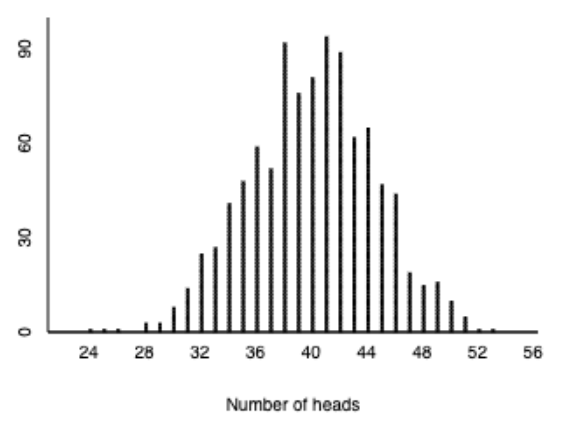
\includegraphics[width = 0.5 \linewidth]{sim1.png}
		\end{center}
		\begin{mcanswerslist}
		\answer[correct] No, since 45 is a fairly typical outcome if the color of the winner's uniform was determined by chance alone.
		\answer Yes, since 45 is larger than 40.
		\answer Yes, since the height of the dotplot above 45 is smaller than the height of the dotplot above 40.
		\answer No, since an observed value greater than 45 could just be by random chance.
		\end{mcanswerslist}
		
		\question[follow] Below are three correct conclusions about this situation, and one incorrect conclusion.  Find the incorrect conclusion.
		\begin{mcanswerslist}
		\answer[correct] The results of this study prove that the color of the winner's uniform was determined by chance alone.
		\answer The results of this study are something that could easily have happened if the color of the winner's uniform was determined by chance alone.
		\answer Convincing evidence does not exist against the "by-chance-alone" model.
		\answer Convincing evidence does not exist that red uniform wearers tend to win more often than those wearing blue uniforms.
		\end{mcanswerslist}
		
		\question A test is being performed to see whether a dog, Hope, understands pointing towards an object. Two objects are placed about 2.5 meters away, then the tester point towards one of the objects. In 20 trials, Hope goes to the correct object 13 times (or 65\%).
		Finish filling in the blanks with the correct One Proportion applet inputs to carry out an appropriate simulation of this process, if Hope does not understand pointing towards an object and is just guessing.
		\begin{itemize}
			\item Probability of success: \_\_\_(1)\_\_\_\_
			\item Sample size: \_\_\_(2)\_\_\_\_
			\item Number of samples: 10,000
		\end{itemize}
		\begin{mcanswerslist}
		\answer[correct] 0.5, 20
		\answer 0.65, 13
		\answer 0.65, 20
		\answer 0.5, 13
		\end{mcanswerslist}
		
		\begin{mcquestioninstruction}
			A survey on 1,500 high school seniors who took the SAT and who completed an optional web survey shows that 55\% of high school seniors are fairly certain that they will participate in a study abroad program in college. Does this survey provide convincing evidence that the majority (more than 50\%) of all high school seniors who take the SAT are fairly certain they will participate in a study abroad program in college?
			
			Refer to this scenario for the next three questions
		\end{mcquestioninstruction}
		
		\question What is the value of the statistic and proper notation in this study?
		\begin{mcanswerslist}
			\answer[correct] \(\hat p=0.55\)
			\answer \(\pi=0.55\)
			\answer \(\mu=825\)
			\answer \(\pi=825\)
		\end{mcanswerslist}		
		
		\question[follow] State the null and alternative hypotheses in proper notation.
		\begin{mcanswerslist}
			\answer[correct] \(H_0: \pi = 0.50\) versus \(H_A: \pi > 0.50\)
			\answer \(H_0: \pi = 0.50\) versus \(H_A: \pi = 0.55 \)
			\answer \(H_0: \pi = 0.55\) versus \(H_A: \pi > 0.55\)
			\answer \(H_0: \hat p = 0.50\) versus \(H_A: \hat p > 0.50\)
		\end{mcanswerslist}
		
		\question[follow] The p-value for this study is less than 0.001. Interpret this value in context of the problem.
		\begin{mcanswerslist}
			\answer[correct] In less than 0.1\% of all samples of 1,500 high school seniors who take the SAT, 55\% or more would respond that they are fairly certain they will participate in a study abroad program in college, if the true probability is 0.50.
			\answer There is less than a 0.1\% chance that 50\% of all high school seniors who take the SAT are fairly certain they will participate in a study abroad program in college.
			\answer In less than 0.1\% of all samples of 1,500 high school seniors who take the SAT, 50\% or more would respond that they are fairly certain they will participate in a study abroad program in college, if the true probability is 0.55.
			\answer There is less than a 0.1\% chance that more than 50\% of all high school seniors who take the SAT are fairly certain they will participate in a study abroad program in college.
		\end{mcanswerslist}
		
		\begin{mcquestioninstruction}
			Research done in the mid 1980s indicated that 80\% of grizzly bears in the greater ecosystem of Yellowstone National Park entered their den for hibernation by the last day of November. This has come into question as of late. Researchers have hypothesized that climate change has postponed bears entering hibernation until later in the season; that is, researchers believe that a smaller percentage of bears are entering their den for hibernation by the last day of November. Sixty-two Yellowstone grizzly bears were tracked via radio monitors, which allow scientists to pinpoint when the bears enter their dens with a high degree of accuracy. Of the sixty-two Yellowstone grizzly bears being tracked, forty-two entered their den for hibernation by the last day of November.
			
			Refer to this scenario for the next two questions
		\end{mcquestioninstruction}
		
		\question[follow] What values would be entered for each of the following in the One Proportion applet to conduct a simulation-based hypothesis test with these data?
		\begin{itemize}
			\item Probability of success: \_\_\_(1)\_\_\_\_
			\item Sample size: \_\_\_(2)\_\_\_\_
			\item Number of samples: Any integer at least 1000
		\end{itemize}
		\begin{mcanswerslist}
			\answer[correct] 0.8, 62
			\answer 0.5, 80
			\answer 0.5, 62
			\answer 0.8, 80
		\end{mcanswerslist}
		
		\question[follow] The simulation-based p-value for this test is 0.0153. Which of the following conclusions are correct?
		\begin{mcanswerslist}
			\answer[correct] Strong evidence exists in favor of the alternative hypothesis.
			\answer Little to no evidence exists against the null hypothesis.
			\answer Strong evidence exists in favor of the null hypothesis.
			\answer Little to no evidence exists against the alternative hypothesis.
		\end{mcanswerslist}
		
	\end{mcquestions}
\end{document}